\documentclass{standalone}
\usepackage{tikz}
\usetikzlibrary{patterns, positioning}


\begin{document}
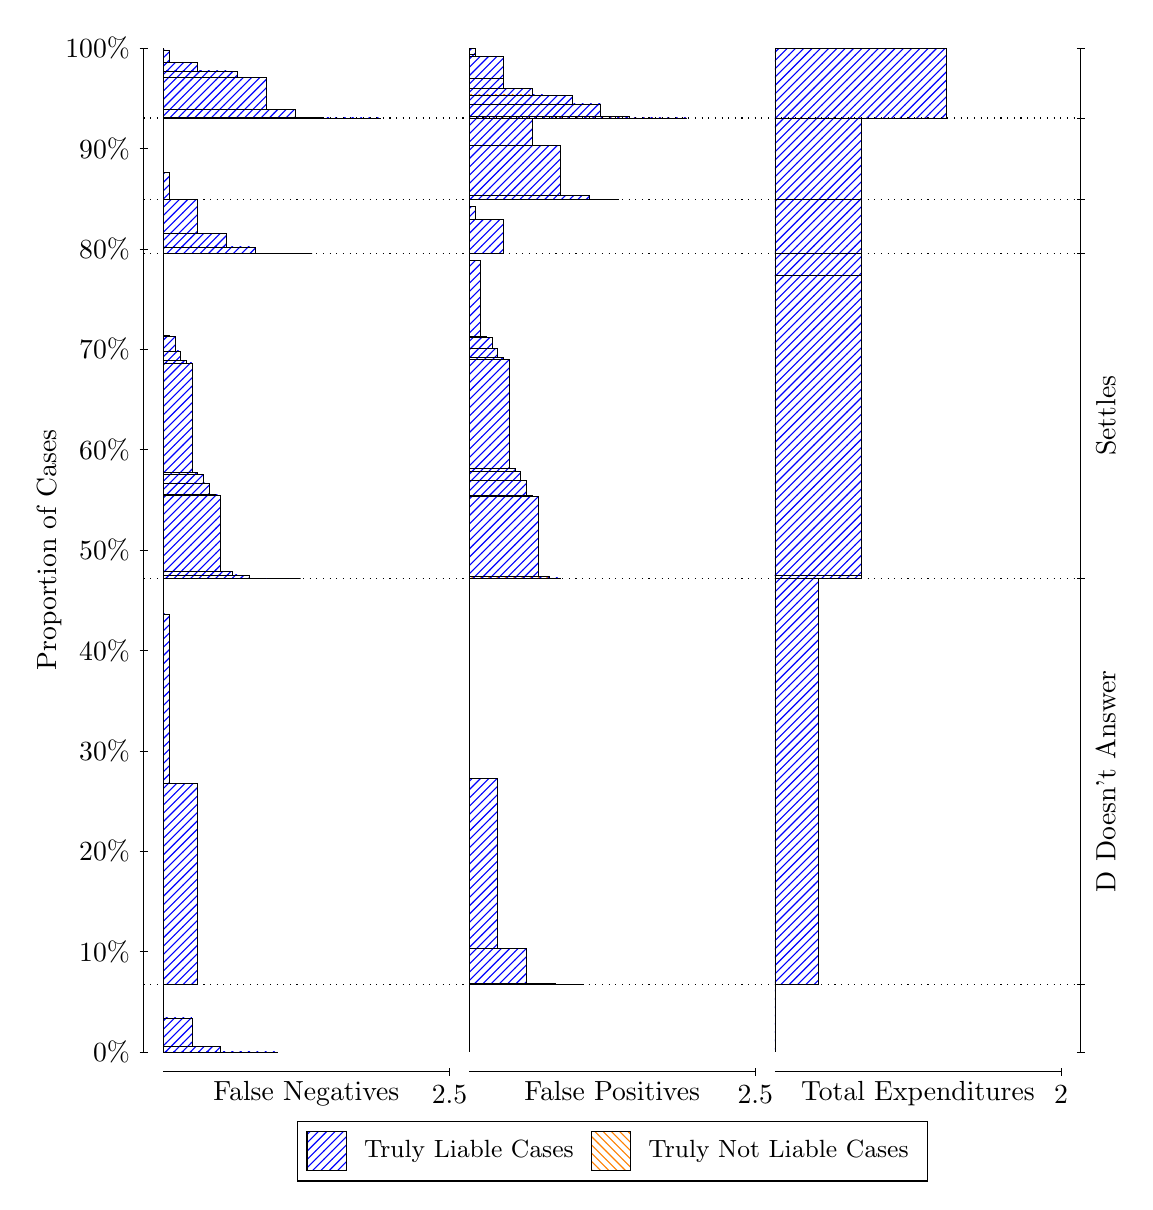
\begin{tikzpicture}
\draw[black, very thin] (1.5,1.75) -- (1.5,14.5);
\node[rotate=90, text=black, anchor=center] at (0.3, 8.125) {Proportion of Cases};
\draw[black, very thin] (1.45,1.75) -- (1.55,1.75);
\node[text=black, anchor=east] at (1.45, 1.75) {0\%};
\draw[black, very thin] (1.45,3.025) -- (1.55,3.025);
\node[text=black, anchor=east] at (1.45, 3.025) {10\%};
\draw[black, very thin] (1.45,4.3) -- (1.55,4.3);
\node[text=black, anchor=east] at (1.45, 4.3) {20\%};
\draw[black, very thin] (1.45,5.575) -- (1.55,5.575);
\node[text=black, anchor=east] at (1.45, 5.575) {30\%};
\draw[black, very thin] (1.45,6.85) -- (1.55,6.85);
\node[text=black, anchor=east] at (1.45, 6.85) {40\%};
\draw[black, very thin] (1.45,8.125) -- (1.55,8.125);
\node[text=black, anchor=east] at (1.45, 8.125) {50\%};
\draw[black, very thin] (1.45,9.4) -- (1.55,9.4);
\node[text=black, anchor=east] at (1.45, 9.4) {60\%};
\draw[black, very thin] (1.45,10.675) -- (1.55,10.675);
\node[text=black, anchor=east] at (1.45, 10.675) {70\%};
\draw[black, very thin] (1.45,11.95) -- (1.55,11.95);
\node[text=black, anchor=east] at (1.45, 11.95) {80\%};
\draw[black, very thin] (1.45,13.225) -- (1.55,13.225);
\node[text=black, anchor=east] at (1.45, 13.225) {90\%};
\draw[black, very thin] (1.45,14.5) -- (1.55,14.5);
\node[text=black, anchor=east] at (1.45, 14.5) {100\%};

\draw[black, very thin] (13.4,1.75) -- (13.4,14.5);
\draw[black, very thin] (13.35,1.75) -- (13.45,1.75);
\node[anchor=west] at (13.35, 1.75) {};
\draw[black, very thin] (13.35,2.6123) -- (13.45,2.6123);
\node[anchor=west] at (13.35, 2.6123) {};
\draw[black, very thin] (13.35,7.7674) -- (13.45,7.7674);
\node[anchor=west] at (13.35, 7.7674) {};
\draw[black, very thin] (13.35,11.893) -- (13.45,11.893);
\node[anchor=west] at (13.35, 11.893) {};
\draw[black, very thin] (13.35,12.573) -- (13.45,12.573);
\node[anchor=west] at (13.35, 12.573) {};
\draw[black, very thin] (13.35,13.612) -- (13.45,13.612);
\node[anchor=west] at (13.35, 13.612) {};
\draw[black, very thin] (13.35,14.5) -- (13.45,14.5);
\node[anchor=west] at (13.35, 14.5) {};

\draw[black, very thin, pattern color=blue, pattern=north east lines] (1.75,1.75) rectangle (3.2033,1.75);
\draw[black, very thin, pattern color=blue, pattern=north east lines] (1.75,1.75) rectangle (2.84,1.7506);
\draw[black, very thin, pattern color=blue, pattern=north east lines] (1.75,1.7506) rectangle (2.4767,1.819);
\draw[black, very thin, pattern color=blue, pattern=north east lines] (1.75,1.819) rectangle (2.1133,2.1817);
\draw[black, very thin, pattern color=orange, pattern=north west lines] (1.75,2.1817) rectangle (1.75,2.1817);
\draw[black, very thin, pattern color=blue, pattern=north east lines] (1.75,2.1817) rectangle (1.75,2.6123);
\draw[black, very thin, pattern color=blue, pattern=north east lines] (1.75,2.6123) rectangle (2.186,5.1582);
\draw[black, very thin, pattern color=blue, pattern=north east lines] (1.75,5.1582) rectangle (1.8227,7.3138);
\draw[black, very thin, pattern color=orange, pattern=north west lines] (1.75,7.3138) rectangle (1.75,7.3138);
\draw[black, very thin, pattern color=blue, pattern=north east lines] (1.75,7.3138) rectangle (1.75,7.7674);
\draw[black, very thin, pattern color=blue, pattern=north east lines] (1.75,7.7674) rectangle (3.494,7.7674);
\draw[black, very thin, pattern color=blue, pattern=north east lines] (1.75,7.7674) rectangle (3.3487,7.7674);
\draw[black, very thin, pattern color=blue, pattern=north east lines] (1.75,7.7674) rectangle (3.2033,7.7674);
\draw[black, very thin, pattern color=blue, pattern=north east lines] (1.75,7.7674) rectangle (3.1307,7.7674);
\draw[black, very thin, pattern color=blue, pattern=north east lines] (1.75,7.7674) rectangle (3.058,7.7674);
\draw[black, very thin, pattern color=blue, pattern=north east lines] (1.75,7.7674) rectangle (2.9853,7.7689);
\draw[black, very thin, pattern color=blue, pattern=north east lines] (1.75,7.7689) rectangle (2.9127,7.7689);
\draw[black, very thin, pattern color=blue, pattern=north east lines] (1.75,7.7689) rectangle (2.84,7.8026);
\draw[black, very thin, pattern color=blue, pattern=north east lines] (1.75,7.8026) rectangle (2.7673,7.8029);
\draw[black, very thin, pattern color=blue, pattern=north east lines] (1.75,7.8029) rectangle (2.6947,7.8086);
\draw[black, very thin, pattern color=blue, pattern=north east lines] (1.75,7.8086) rectangle (2.622,7.8555);
\draw[black, very thin, pattern color=blue, pattern=north east lines] (1.75,7.8555) rectangle (2.5493,7.8564);
\draw[black, very thin, pattern color=blue, pattern=north east lines] (1.75,7.8564) rectangle (2.4767,8.8241);
\draw[black, very thin, pattern color=blue, pattern=north east lines] (1.75,8.8241) rectangle (2.404,8.8303);
\draw[black, very thin, pattern color=blue, pattern=north east lines] (1.75,8.8303) rectangle (2.3313,8.9777);
\draw[black, very thin, pattern color=blue, pattern=north east lines] (1.75,8.9777) rectangle (2.2587,9.0882);
\draw[black, very thin, pattern color=blue, pattern=north east lines] (1.75,9.0882) rectangle (2.186,9.1106);
\draw[black, very thin, pattern color=blue, pattern=north east lines] (1.75,9.1106) rectangle (2.1133,10.502);
\draw[black, very thin, pattern color=blue, pattern=north east lines] (1.75,10.502) rectangle (2.0407,10.538);
\draw[black, very thin, pattern color=blue, pattern=north east lines] (1.75,10.538) rectangle (1.968,10.653);
\draw[black, very thin, pattern color=blue, pattern=north east lines] (1.75,10.653) rectangle (1.8953,10.838);
\draw[black, very thin, pattern color=blue, pattern=north east lines] (1.75,10.838) rectangle (1.8227,10.849);
\draw[black, very thin, pattern color=orange, pattern=north west lines] (1.75,10.849) rectangle (1.75,10.849);
\draw[black, very thin, pattern color=blue, pattern=north east lines] (1.75,10.849) rectangle (1.75,11.893);
\draw[black, very thin, pattern color=blue, pattern=north east lines] (1.75,11.893) rectangle (3.6393,11.893);
\draw[black, very thin, pattern color=blue, pattern=north east lines] (1.75,11.893) rectangle (3.276,11.896);
\draw[black, very thin, pattern color=blue, pattern=north east lines] (1.75,11.896) rectangle (2.9127,11.975);
\draw[black, very thin, pattern color=blue, pattern=north east lines] (1.75,11.975) rectangle (2.5493,12.142);
\draw[black, very thin, pattern color=blue, pattern=north east lines] (1.75,12.142) rectangle (2.186,12.573);
\draw[black, very thin, pattern color=orange, pattern=north west lines] (1.75,12.573) rectangle (1.75,12.573);
\draw[black, very thin, pattern color=blue, pattern=north east lines] (1.75,12.573) rectangle (2.186,12.577);
\draw[black, very thin, pattern color=blue, pattern=north east lines] (1.75,12.577) rectangle (1.8227,12.924);
\draw[black, very thin, pattern color=orange, pattern=north west lines] (1.75,12.924) rectangle (1.75,12.924);
\draw[black, very thin, pattern color=blue, pattern=north east lines] (1.75,12.924) rectangle (1.75,13.612);
\draw[black, very thin, pattern color=blue, pattern=north east lines] (1.75,13.612) rectangle (4.5113,13.612);
\draw[black, very thin, pattern color=blue, pattern=north east lines] (1.75,13.612) rectangle (4.148,13.612);
\draw[black, very thin, pattern color=blue, pattern=north east lines] (1.75,13.612) rectangle (3.7847,13.615);
\draw[black, very thin, pattern color=blue, pattern=north east lines] (1.75,13.615) rectangle (3.4213,13.721);
\draw[black, very thin, pattern color=blue, pattern=north east lines] (1.75,13.721) rectangle (3.276,13.721);
\draw[black, very thin, pattern color=blue, pattern=north east lines] (1.75,13.721) rectangle (3.058,14.123);
\draw[black, very thin, pattern color=blue, pattern=north east lines] (1.75,14.123) rectangle (2.9127,14.123);
\draw[black, very thin, pattern color=blue, pattern=north east lines] (1.75,14.123) rectangle (2.6947,14.206);
\draw[black, very thin, pattern color=blue, pattern=north east lines] (1.75,14.206) rectangle (2.5493,14.209);
\draw[black, very thin, pattern color=blue, pattern=north east lines] (1.75,14.209) rectangle (2.3313,14.209);
\draw[black, very thin, pattern color=blue, pattern=north east lines] (1.75,14.209) rectangle (2.186,14.209);
\draw[black, very thin, pattern color=blue, pattern=north east lines] (1.75,14.209) rectangle (2.186,14.321);
\draw[black, very thin, pattern color=blue, pattern=north east lines] (1.75,14.321) rectangle (1.8227,14.322);
\draw[black, very thin, pattern color=blue, pattern=north east lines] (1.75,14.322) rectangle (1.8227,14.477);
\draw[black, very thin, pattern color=orange, pattern=north west lines] (1.75,14.477) rectangle (1.75,14.477);
\draw[black, very thin, pattern color=blue, pattern=north east lines] (1.75,14.477) rectangle (1.75,14.5);
\draw[black, very thin, pattern color=orange, pattern=north west lines] (5.6333,1.75) rectangle (5.6333,1.75);
\draw[black, very thin, pattern color=blue, pattern=north east lines] (5.6333,1.75) rectangle (5.6333,2.6123);
\draw[black, very thin, pattern color=orange, pattern=north west lines] (5.6333,2.6123) rectangle (7.0867,2.6123);
\draw[black, very thin, pattern color=blue, pattern=north east lines] (5.6333,2.6123) rectangle (7.0867,2.6124);
\draw[black, very thin, pattern color=blue, pattern=north east lines] (5.6333,2.6124) rectangle (6.7233,2.6249);
\draw[black, very thin, pattern color=blue, pattern=north east lines] (5.6333,2.6249) rectangle (6.36,3.0659);
\draw[black, very thin, pattern color=blue, pattern=north east lines] (5.6333,3.0659) rectangle (5.9967,5.2215);
\draw[black, very thin, pattern color=blue, pattern=north east lines] (5.6333,5.2215) rectangle (5.6333,7.7674);
\draw[black, very thin, pattern color=orange, pattern=north west lines] (5.6333,7.7674) rectangle (6.796,7.7674);
\draw[black, very thin, pattern color=blue, pattern=north east lines] (5.6333,7.7674) rectangle (6.796,7.7704);
\draw[black, very thin, pattern color=orange, pattern=north west lines] (5.6333,7.7704) rectangle (6.6507,7.7704);
\draw[black, very thin, pattern color=blue, pattern=north east lines] (5.6333,7.7704) rectangle (6.6507,7.7877);
\draw[black, very thin, pattern color=orange, pattern=north west lines] (5.6333,7.7877) rectangle (6.5053,7.7877);
\draw[black, very thin, pattern color=blue, pattern=north east lines] (5.6333,7.7877) rectangle (6.5053,8.8118);
\draw[black, very thin, pattern color=blue, pattern=north east lines] (5.6333,8.8118) rectangle (6.4327,8.8229);
\draw[black, very thin, pattern color=orange, pattern=north west lines] (5.6333,8.8229) rectangle (6.36,8.8229);
\draw[black, very thin, pattern color=blue, pattern=north east lines] (5.6333,8.8229) rectangle (6.36,9.0079);
\draw[black, very thin, pattern color=blue, pattern=north east lines] (5.6333,9.0079) rectangle (6.2873,9.1227);
\draw[black, very thin, pattern color=orange, pattern=north west lines] (5.6333,9.1227) rectangle (6.2147,9.1227);
\draw[black, very thin, pattern color=blue, pattern=north east lines] (5.6333,9.1227) rectangle (6.2147,9.1591);
\draw[black, very thin, pattern color=blue, pattern=north east lines] (5.6333,9.1591) rectangle (6.142,10.55);
\draw[black, very thin, pattern color=blue, pattern=north east lines] (5.6333,10.55) rectangle (6.0693,10.572);
\draw[black, very thin, pattern color=blue, pattern=north east lines] (5.6333,10.572) rectangle (5.9967,10.683);
\draw[black, very thin, pattern color=blue, pattern=north east lines] (5.6333,10.683) rectangle (5.924,10.83);
\draw[black, very thin, pattern color=blue, pattern=north east lines] (5.6333,10.83) rectangle (5.8513,10.837);
\draw[black, very thin, pattern color=blue, pattern=north east lines] (5.6333,10.837) rectangle (5.7787,11.804);
\draw[black, very thin, pattern color=blue, pattern=north east lines] (5.6333,11.804) rectangle (5.706,11.805);
\draw[black, very thin, pattern color=blue, pattern=north east lines] (5.6333,11.805) rectangle (5.6333,11.893);
\draw[black, very thin, pattern color=orange, pattern=north west lines] (5.6333,11.893) rectangle (6.0693,11.893);
\draw[black, very thin, pattern color=blue, pattern=north east lines] (5.6333,11.893) rectangle (6.0693,12.324);
\draw[black, very thin, pattern color=blue, pattern=north east lines] (5.6333,12.324) rectangle (5.706,12.491);
\draw[black, very thin, pattern color=blue, pattern=north east lines] (5.6333,12.491) rectangle (5.6333,12.573);
\draw[black, very thin, pattern color=orange, pattern=north west lines] (5.6333,12.573) rectangle (7.5227,12.573);
\draw[black, very thin, pattern color=blue, pattern=north east lines] (5.6333,12.573) rectangle (7.5227,12.574);
\draw[black, very thin, pattern color=blue, pattern=north east lines] (5.6333,12.574) rectangle (7.1593,12.631);
\draw[black, very thin, pattern color=blue, pattern=north east lines] (5.6333,12.631) rectangle (6.796,13.262);
\draw[black, very thin, pattern color=blue, pattern=north east lines] (5.6333,13.262) rectangle (6.4327,13.608);
\draw[black, very thin, pattern color=blue, pattern=north east lines] (5.6333,13.608) rectangle (6.0693,13.612);
\draw[black, very thin, pattern color=orange, pattern=north west lines] (5.6333,13.612) rectangle (8.3947,13.612);
\draw[black, very thin, pattern color=blue, pattern=north east lines] (5.6333,13.612) rectangle (8.3947,13.612);
\draw[black, very thin, pattern color=orange, pattern=north west lines] (5.6333,13.612) rectangle (8.0313,13.612);
\draw[black, very thin, pattern color=blue, pattern=north east lines] (5.6333,13.612) rectangle (8.0313,13.613);
\draw[black, very thin, pattern color=orange, pattern=north west lines] (5.6333,13.613) rectangle (7.668,13.613);
\draw[black, very thin, pattern color=blue, pattern=north east lines] (5.6333,13.613) rectangle (7.668,13.636);
\draw[black, very thin, pattern color=orange, pattern=north west lines] (5.6333,13.636) rectangle (7.3047,13.636);
\draw[black, very thin, pattern color=blue, pattern=north east lines] (5.6333,13.636) rectangle (7.3047,13.791);
\draw[black, very thin, pattern color=blue, pattern=north east lines] (5.6333,13.791) rectangle (6.9413,13.903);
\draw[black, very thin, pattern color=orange, pattern=north west lines] (5.6333,13.903) rectangle (6.796,13.903);
\draw[black, very thin, pattern color=blue, pattern=north east lines] (5.6333,13.903) rectangle (6.796,13.903);
\draw[black, very thin, pattern color=blue, pattern=north east lines] (5.6333,13.903) rectangle (6.578,13.906);
\draw[black, very thin, pattern color=orange, pattern=north west lines] (5.6333,13.906) rectangle (6.4327,13.906);
\draw[black, very thin, pattern color=blue, pattern=north east lines] (5.6333,13.906) rectangle (6.4327,13.989);
\draw[black, very thin, pattern color=blue, pattern=north east lines] (5.6333,13.989) rectangle (6.2147,13.989);
\draw[black, very thin, pattern color=blue, pattern=north east lines] (5.6333,13.989) rectangle (6.0693,14.111);
\draw[black, very thin, pattern color=orange, pattern=north west lines] (5.6333,14.111) rectangle (6.0693,14.111);
\draw[black, very thin, pattern color=blue, pattern=north east lines] (5.6333,14.111) rectangle (6.0693,14.391);
\draw[black, very thin, pattern color=blue, pattern=north east lines] (5.6333,14.391) rectangle (5.8513,14.391);
\draw[black, very thin, pattern color=blue, pattern=north east lines] (5.6333,14.391) rectangle (5.706,14.422);
\draw[black, very thin, pattern color=blue, pattern=north east lines] (5.6333,14.422) rectangle (5.706,14.497);
\draw[black, very thin, pattern color=blue, pattern=north east lines] (5.6333,14.497) rectangle (5.6333,14.5);
\draw[black, very thin, pattern color=orange, pattern=north west lines] (9.5167,1.75) rectangle (9.5167,1.75);
\draw[black, very thin, pattern color=blue, pattern=north east lines] (9.5167,1.75) rectangle (9.5167,2.6123);
\draw[black, very thin, pattern color=orange, pattern=north west lines] (9.5167,2.6123) rectangle (10.062,2.6123);
\draw[black, very thin, pattern color=blue, pattern=north east lines] (9.5167,2.6123) rectangle (10.062,7.7674);
\draw[black, very thin, pattern color=orange, pattern=north west lines] (9.5167,7.7674) rectangle (10.607,7.7674);
\draw[black, very thin, pattern color=blue, pattern=north east lines] (9.5167,7.7674) rectangle (10.607,7.8049);
\draw[black, very thin, pattern color=orange, pattern=north west lines] (9.5167,7.8049) rectangle (10.607,7.8049);
\draw[black, very thin, pattern color=blue, pattern=north east lines] (9.5167,7.8049) rectangle (10.607,11.608);
\draw[black, very thin, pattern color=orange, pattern=north west lines] (9.5167,11.608) rectangle (10.607,11.608);
\draw[black, very thin, pattern color=blue, pattern=north east lines] (9.5167,11.608) rectangle (10.607,11.893);
\draw[black, very thin, pattern color=orange, pattern=north west lines] (9.5167,11.893) rectangle (10.607,11.893);
\draw[black, very thin, pattern color=blue, pattern=north east lines] (9.5167,11.893) rectangle (10.607,12.573);
\draw[black, very thin, pattern color=orange, pattern=north west lines] (9.5167,12.573) rectangle (10.607,12.573);
\draw[black, very thin, pattern color=blue, pattern=north east lines] (9.5167,12.573) rectangle (10.607,13.612);
\draw[black, very thin, pattern color=orange, pattern=north west lines] (9.5167,13.612) rectangle (11.697,13.612);
\draw[black, very thin, pattern color=blue, pattern=north east lines] (9.5167,13.612) rectangle (11.697,14.5);
\draw[black, dotted] (1.5,2.6123) -- (13.4,2.6123);
\draw[black, dotted] (1.5,7.7674) -- (13.4,7.7674);
\draw[black, dotted] (1.5,11.893) -- (13.4,11.893);
\draw[black, dotted] (1.5,12.573) -- (13.4,12.573);
\draw[black, dotted] (1.5,13.612) -- (13.4,13.612);
\draw[black, very thin] (1.75,1.5) -- (5.3833,1.5);
\node[text=black, anchor=north] at (3.5667, 1.5) {False Negatives};
\draw[black, very thin] (5.3833,1.45) -- (5.3833,1.55);
\node[text=black, anchor=north] at (5.3833, 1.45) {2.5};

\draw[black, very thin] (5.6333,1.5) -- (9.2667,1.5);
\node[text=black, anchor=north] at (7.45, 1.5) {False Positives};
\draw[black, very thin] (9.2667,1.45) -- (9.2667,1.55);
\node[text=black, anchor=north] at (9.2667, 1.45) {2.5};

\draw[black, very thin] (9.5167,1.5) -- (13.15,1.5);
\node[text=black, anchor=north] at (11.333, 1.5) {Total Expenditures};
\draw[black, very thin] (13.15,1.45) -- (13.15,1.55);
\node[text=black, anchor=north] at (13.15, 1.45) {2};


\node[text=black, centered, rotate=90] at (13.72, 5.1899) {D Doesn't Answer};
\node[text=black, centered, rotate=90] at (13.72, 9.8303) {Settles};




\draw (7.449999999999999,1.5) node[draw=none] (baseCoordinate) {};
\begin{scope}[align=center]
        \matrix[scale=0.5, draw=black, below=0.5cm of baseCoordinate, nodes={draw}, column sep=0.1cm]{
            \node[rectangle, draw, minimum width=0.5cm, minimum height=0.5cm, pattern color=blue, pattern=north east lines] {}; &
            \node[draw=none, font=\small, text=black] (B) {Truly Liable Cases}; &
            \node[rectangle, draw, minimum width=0.5cm, minimum height=0.5cm, pattern color=orange, pattern=north west lines] {}; &
            \node[draw=none, font=\small, text=black] (B) {Truly Not Liable Cases}; \\
            };
\end{scope}

\end{tikzpicture}
\end{document}